\documentclass[a4paper,10pt]{scrbook}
\usepackage[italian]{babel}
\usepackage[utf8x]{inputenc}
\usepackage{amsmath}
\usepackage{amsthm}
\usepackage{amssymb}
\usepackage{amscd}
\usepackage{graphicx}
\usepackage{float}
\usepackage{array}
\usepackage{rotating}
\usepackage{caption}
\usepackage{lscape}
\usepackage{fancybox}

\renewcommand{\fboxsep}{0.5cm}
\usepackage{hyperref}

\hypersetup{
    bookmarks=true,         % show bookmarks bar?
    unicode=false,          % non-Latin characters in Acrobat’s bookmarks
    pdftoolbar=true,        % show Acrobat’s toolbar?
    pdfmenubar=true,        % show Acrobat’s menu?
    pdffitwindow=false,     % window fit to page when opened
    pdfstartview={FitH},    % fits the width of the page to the window
    pdftitle={Sigurd  Cms},    % title
    pdfauthor={Matteo Mosangini},     % author
    pdfsubject={Gestione Cms scolastico},   % subject of the document
    pdfcreator={Matteo Mosangini},   % creator of the document
    pdfproducer={Matteo Mosangini}, % producer of the document
    pdfkeywords={cms ezpublish sigurd scuola alunni}, % list of keywords
    pdfnewwindow=true,      % links in new window
    colorlinks=false,       % false: boxed links; true: colored links
    linkcolor=red,          % color of internal links
    citecolor=green,        % color of links to bibliography
    filecolor=magenta,      % color of file links
    urlcolor=cyan           % color of external links
}

\renewcommand{\textfraction}{0.05}
\renewcommand{\topfraction}{0.95}
\renewcommand{\bottomfraction}{0.95}
\renewcommand{\floatpagefraction}{0.35}
\setcounter{totalnumber}{5}
\restylefloat{figure}
\newlength{\drop}


\newcommand{\titleBWF}{\begingroup% Beowulf
\drop = 0.1\textheight
\parindent=0pt
\vspace{\drop}
{\Huge\bfseries Cms Scolastico - mini guida}\\[\baselineskip]
{\Large {\itshape Guida} {\scshape per i docenti}}\par
\vspace{5cm}
\begin{center}
\includegraphics[width=0.4\textwidth]{./immagini/logo/sigurd2.png}
\end{center}
\centering
{\Huge\bfseries S.I.G.U.R.D}\footnote{Sistema integrato gestione unificata risorse didattiche}

{\Large\itshape }
\vspace*{\drop}
\endgroup}


\begin{document}




\begin{titlepage}
 \titleBWF
\end{titlepage}

\tableofcontents
\chapter[Registrazione]{La registrazione degli utenti}

Attualmente il sito prevede la presenza di quattro classi di utenti:

\begin{itemize}
 \item Genitori
\item Professori
\item Ata
\item Alunni
\end{itemize}


Dopo aver selezionato il collegamento \emph{Registrati} l'utente ha la possibilità di scegliere tra le classi prima illustrate quella più affine.

\begin{figure}[H]
 \centering
 \includegraphics[width=0.8\textwidth]{./immagini/registrazione/scelta_genere.png}
 % scelta_genere.png: 524x362 pixel, 72dpi, 18.49x12.77 cm, bb=
 \caption{Selezione del tipo di utente}
 \label{fig:reg_sel}
\end{figure}
Per ogni classe di utenti verrà presentata dal sistema una diversa form dedicata all'inserimento dei dati personali:
\begin{itemize}
 \item Genitori
\begin{itemize}
 \item Nome, Cognome, Dati account
\item Scuola frequentata dai figli
\item Figli frequentanti le varie scuole
\end{itemize}
\item Professori
\begin{itemize}
 \item Nome, Cognome, Dati account
\item Scuole di appartenenza
\item Classi di docenza
\item Sedi geografice di insegnamento
\end{itemize}
\item Ata
\begin{itemize}
 \item Nome, Cognome, Dati account
\item Scuole di appartenenza
\item Mansione
\end{itemize}
\item Alunni
\begin{itemize}
 \item Nome, Cognome, Dati account
\item Scuola frequentata
\end{itemize}
\end{itemize}


\section{Registrazione insegnante}

Durante la fase di registrazione l'insegnante è tenuto ad inserire:
\begin{description}
 \item[Nome e cognome] Il proprio nome e cognome con cui l'insegnante potrà essere individuato all'interno dell'istituto
\item[Account] Il sistema richiede il nome utente preferibilmente della forma \textbf{nome.cognome} e la password per accedere al sito. Si consiglia di utilizzare una password alfanumerica.
\item[Firma] Una frase da riportare nel proprio spazio utente
\item[Avatar] Una foto o un disegno rappresentanti l'utente
\item[Istituti] L'istituto o gli istituti in cui l'insegnante lavora
\item[Classi] Le classi di docenza del presente anno scolastico. Le scelte fatte durante il processo di registrazione circa le classi potranno essere modificate in qualsiasi momento
\item[Sede geografica] La sede o le sedi geografiche in cui l'insegnante lavora 
\end{description}

\begin{figure}[H]
 \centering
 \includegraphics[width=\textwidth]{./immagini/registrazione/registrazione_prof1.png}
 % registrazione_prof1.png: 1126x621 pixel, 72dpi, 39.72x21.91 cm, bb=
 \caption{Inserimento del nome cognome e dei dati account}
 \label{fig:reg_prof1}
\end{figure}
\begin{figure}[H]
 \centering
 \includegraphics[width=\textwidth]{./immagini/registrazione/registrazione_prof2.png}
 % registrazione_prof2.png: 855x687 pixel, 72dpi, 30.16x24.24 cm, bb=
 \caption{Scelta delle scuole}
 \label{fig:reg_prof2}
\end{figure}


\begin{figure}[H]
 \centering
 \includegraphics[width=\textwidth,bb=0 0 760 158]{./immagini/registrazione/registrazione_prof3.png}
 % registrazione_prof3.png: 760x158 pixel, 72dpi, 26.81x5.57 cm, bb=0 0 760 158
 \caption{Scelta delle materie e della sede geografica}
 \label{fig:reg_prof3}
\end{figure}
\section{Registrazione ata}

Per effettuare la registrazione un membro del personale Ata dovrà completare i seguenti campi:

\begin{description}
 \item[Nome e cognome] Il proprio nome e cognome con cui l'insegnante potrà essere individuato all'interno dell'istituto
\item[Account] Il sistema richiede il nome utente preferibilmente della forma \textbf{nome.cognome} e la password per accedere al sito. Si consiglia di utilizzare una password alfanumerica.
\item[Firma] Una frase da riportare nel proprio spazio utente
\item[Avatar] Una foto o un disegno rappresentanti l'utente
\item[Istituti] L'istituto o gli istituti in cui l'insegnante lavora
\item[Mansioni] Le mansioni svolte all'interno dell'istituto
\end{description}


 \begin{figure}[H]
 \centering
 \includegraphics[width=\textwidth]{./immagini/registrazione/ata_reg_1.png}
 % ata_reg_1.png: 763x156 pixel, 72dpi, 26.92x5.50 cm, bb=
 \caption{Scelta della mansione durante la registrazione}
 \label{fig:reg_ata1}
\end{figure}



\section{Registrazione genitori}

Per effettuare la registrazione i genitori dovranno complatare i seguenti campi:

\begin{description}
 \item[Nome e cognome] Il proprio nome e cognome con cui l'insegnante potrà essere individuato all'interno dell'istituto
\item[Account] Il sistema richiede il nome utente preferibilmente della forma \textbf{nome.cognome} e la password per accedere al sito. Si consiglia di utilizzare una password alfanumerica.
\item[Firma] Una frase da riportare nel proprio spazio utente
\item[Avatar] Una foto o un disegno rappresentanti l'utente
\item[Istituti] L'istituto o gli istituti in cui si trovano i figli
\item[Figli] Elenco dei figli con corrispondente scuola di appartenenza
\end{description}

\begin{figure}[H]
 \centering
 \includegraphics[width=\textwidth]{./immagini/registrazione/genitore_reg_1.png}
 % genitore_reg_1.png: 770x254 pixel, 72dpi, 27.16x8.96 cm, bb=
 \caption{Inserimento dei figli con relativa scuola di appartenenza}
 \label{fig:reg_gen1}
\end{figure}

\section{Registrazione Alunni}

Per effettuare la registrazione gli alunni dovranno complatare i seguenti campi:

\begin{description}
 \item[Nome e cognome] Il proprio nome e cognome con cui l'insegnante potrà essere individuato all'interno dell'istituto
\item[Account] Il sistema richiede il nome utente preferibilmente della forma \textbf{nome.cognome} e la password per accedere al sito. Si consiglia di utilizzare una password alfanumerica.
\item[Firma] Una frase da riportare nel proprio spazio utente
\item[Avatar] Una foto o un disegno rappresentanti l'utente
\item[Istituti] L'istituto in cui studi

\end{description}
\section{Procedure successiva alla registrazione}

Dopo aver concluso il processo ed inviato il formulario al server, vi verrà recapitata una e-mail (dovreste riceverla in pochi secondi). All'interno di questa e-mail troverete un link, seguitelo cliccandoci sopra con il mouse. Il vostro account viene quindi confermato. Come da indicazioni a monitor stampata l'email appena ricevuta e portatela a scuola, in questo modo avremo la certezza che soltanto i membri dell'istituto abbiano accesso alle parti riservate del sito. Non appena il vostro account sarà attivato riceverete automaticamente un'email.



\chapter[Gestione professori]{Professori: gestione spazio personale}


\begin{figure}[H]
 \centering
 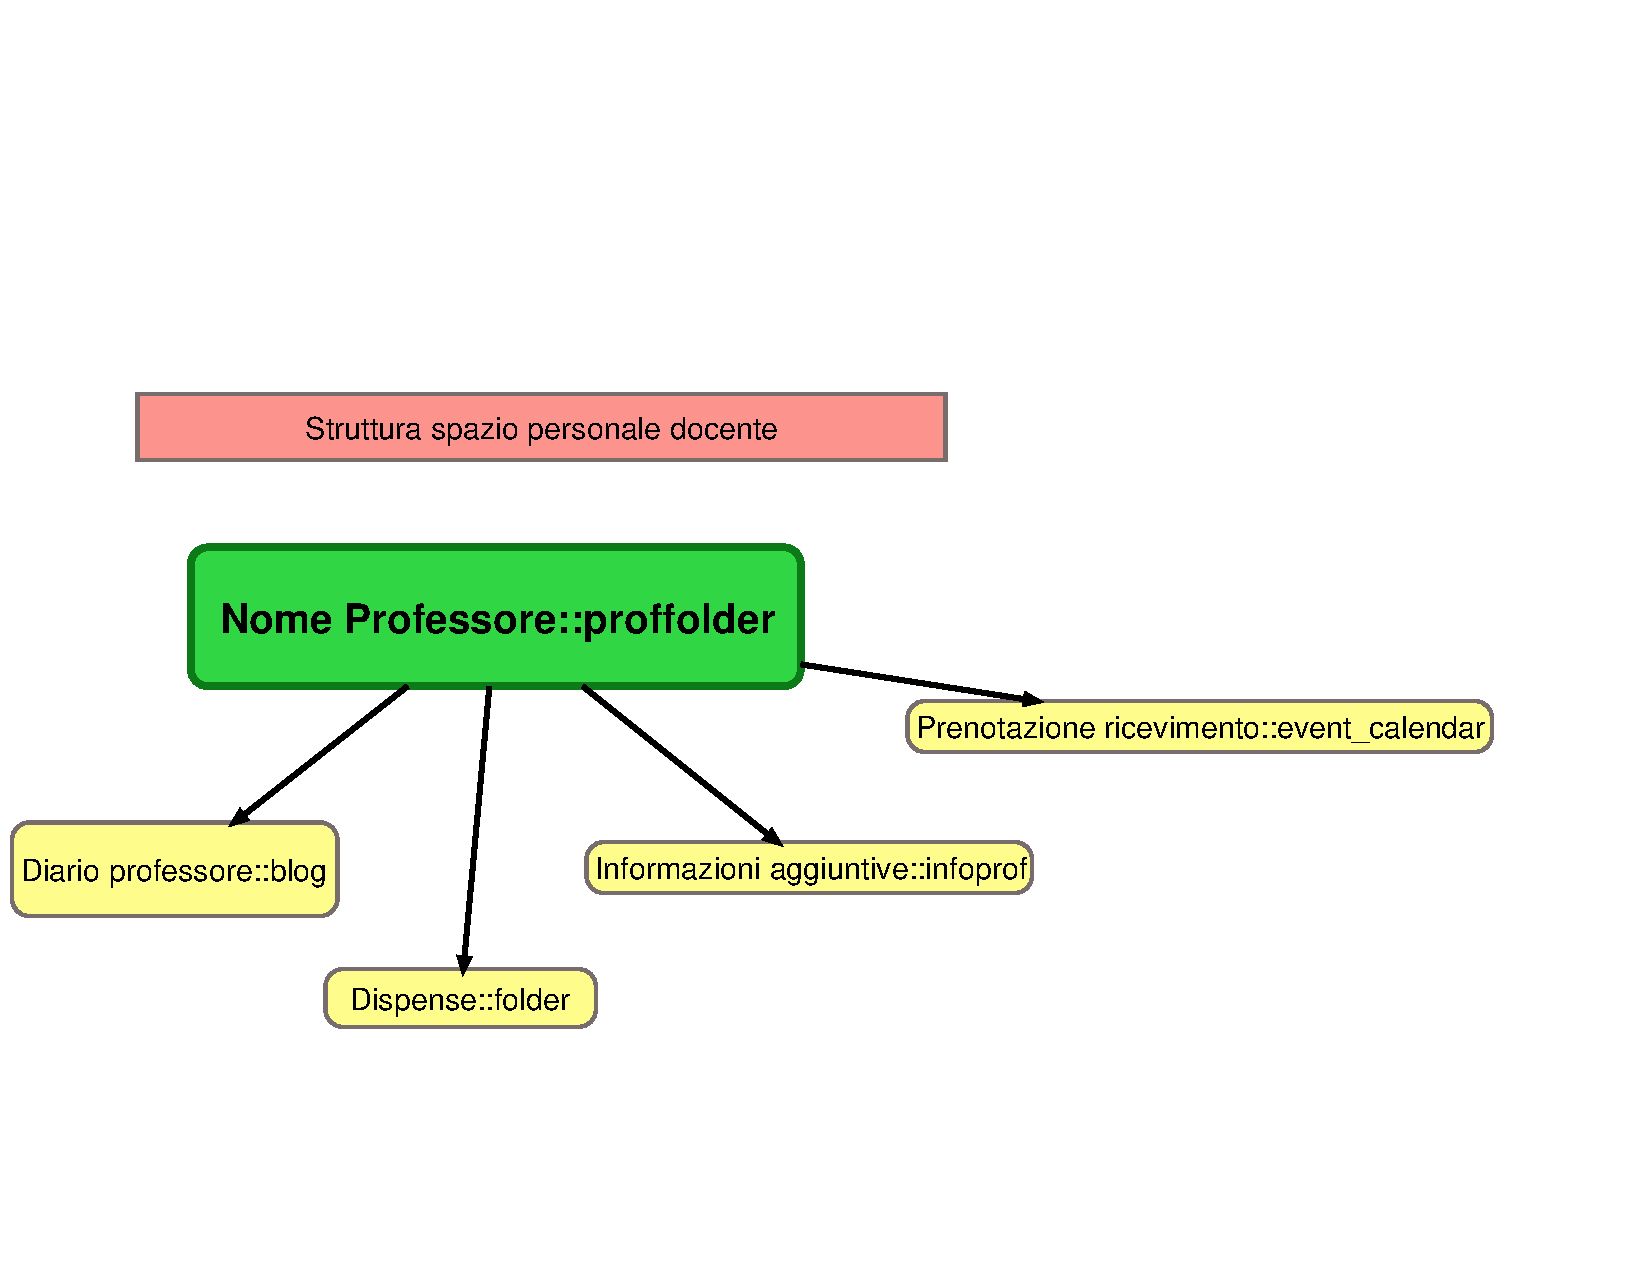
\includegraphics[width=\textwidth]{./immagini/prof_guide/struttura_spazio_docente.pdf}
 % struttura_spazio_docente.pdf: 792x612 pixel, 72dpi, 27.94x21.59 cm, bb=
 \caption{Struttura dello spazio docente creata durante la fase di registrazione}
 \label{fig:proffolder_structture}
\end{figure}



Ogni docente ha a disposizione uno  (o più) spazi personali all'interno dei quali può caricare contenuti utili all'attività didattica. La Collocazione di ogni spazio personale è:
\begin{verbatim}
 \Home\<Nome scuola>\Docenti\<Nome docente>
\end{verbatim}
se un insegnante lavora in più scuole gestite dall'istituto in ognuna di queste avrà a disposizione uno spazio personale diversificato in cui inserire i suoi contenuti.

\begin{figure}[H]
 \centering
 \includegraphics[width=\textwidth]{./immagini/prof_guide/user_links.png}
 % user_links.png: 578x38 pixel, 72dpi, 20.39x1.34 cm, bb=
 \caption{Link accessibili all'utente registrato}
 \label{fig:user_links}
\end{figure}

Oltre allo spazio personale ogni insegnate dispone di un profilo personale, non visibile pubblicamente, tramite il quale può gestire le sue relazione con la struttura scolastica (classi di insegnamento, plessi di insegnamento, collocazione geografica della sede di lavoro). Per accedere al profilo personale è sufficiente, una volta effettuato il login, cliccare con il mouse sui link presenti nella parte alta della pagina figura.\ref{fig:user_links}

Verrà quindi visualizzato il profilo personale. In  tal pagina sarà possibile modificare le proprie preferenze operative, cambiare il proprio avatar etc. Nel caso di un insegnate, ovvero di un utente con a disposizione uno spazio personale verranno anche elencati tali spazi figura.\ref{fig:vista_profilo_utente}
\begin{figure}[h]
 \centering
 \includegraphics[width=\textwidth]{./immagini/prof_guide/prof_profile0.png}
 % prof_profile0.png: 1173x590 pixel, 72dpi, 41.38x20.81 cm, bb=
 \caption{Vista generale del profilo utente professore}
 \label{fig:vista_profilo_utente}
\end{figure}

Per modificare il profilo personale è sufficiente cliccare con il mouse sul pulsante \textsl{Modifica}, comparirà la pagina di modifica all'interno della quale andremo ad impostare le preferenze. Figura.\ref{fig:profile_edit1}

\begin{figure}[H]
 \centering
 \includegraphics[width=\textwidth]{./immagini/prof_guide/prof_profil1.png}
 % personal_prof1.png: 1063x421 pixel, 72dpi, 37.50x14.85 cm, bb=
 \caption{Modifica del profilo personale: è possibili modificare i propri dati come nome,cognome, password, indirizzo e-mail}
 \label{fig:profile_edit1}
\end{figure}
È possibile caricare un'immagine che sarà utilizzata nello spazio personale docente e specificare le scuole in cui si insegna. Figura.\ref{fig:profile_edit2}

\begin{figure}[H]
 \centering
 \includegraphics[width=\textwidth]{./immagini/prof_guide/prof_profile_2.png}
 % personal_prof2.png: 1071x111 pixel, 72dpi, 37.78x3.92 cm, bb=
 \caption{È possible caricare una  proprio foto nel profilo utente}
 \label{fig:profile_edit2}
\end{figure}
Quando le classi di insegnamento cambiano è possibile riassociare lo spazio personale insegnante alle nuove classi. Figura.\ref{fig:edit_profile3}

\begin{figure}[H]
 \centering
 \includegraphics[width=\textwidth]{./immagini/prof_guide/prof_profile3.png}
 % prof_profile3.png: 1244x642 pixel, 72dpi, 43.89x22.65 cm, bb=
 \caption{Modifica delle classi di insegnamento}
 \label{fig:edit_profile3}
\end{figure}
\section{Inserimento dati nello spazio personale}

\subsection{Attivazione spazio personale}
Per poter rendere disponibile nella sezione pubblica del sito il proprio spazio personale, dopo l'attivazione il docente deve modificare lo stato dell'oggetto di Classe Prof Folder istanziato durante la creazione dell'account.
Per far questo, dopo aver effettuato il login ed essersi posizionato nella cartella personale:
\begin{verbatim}
 <Scuola>/Docenti/<Nome Docente>
\end{verbatim}

deve cliccare sul tasto:
 \includegraphics[bb=0 0 26 32]{./immagini/edit/tasto_stato.png} 
e nella finestra di dialogo per l'impostazione degli stati selezionare \textsl{Pronto}:
\begin{figure}[H]
 \centering
 \includegraphics[width=\textwidth]{./immagini/prof_guide/stati_docente.png}
 % stati_docente.png: 1245x164 pixel, 72dpi, 43.92x5.79 cm, bb=
 \caption{Impostate lo stato come pronto visualizzare lo spazio personale nella sezione pubblica del sito}
 \label{fig:stati_docente}
\end{figure}





Se l'insegnate ha sufficienti permessi, quando si trova all'interno del suo spazio personale comparirà una barra degli strumenti subito sotto il menu a tendina figura.\ref{fig:toolbar_1}. Tramite questa barra sarà possibile creare dei contenuti all'interno dello spazio personale o modificare quelli già presenti figura.\ref{fig:toolbar_2}.

\begin{figure}[H]
 \centering
 \includegraphics[width=\textwidth]{./immagini/prof_guide/toolbar_1.png}
 % toolbar_1.png: 242x44 pixel, 72dpi, 8.54x1.55 cm, bb=
 \caption{Toolbar per la creazione dei contenuti: scelta della classe}
 \label{fig:toolbar_1}
\end{figure}

\begin{figure}[H]
 \centering
 \includegraphics[width=\textwidth]{./immagini/prof_guide/toolbar2.png}
 % toolbar2.png: 236x51 pixel, 72dpi, 8.33x1.80 cm, bb=
 \caption{Azioni disponibili all'utente}
 \label{fig:toolbar_2}
\end{figure}
Nello spazio personale è possibile inserire dei recapiti diversi da quelli inseriti nel profilo utente. Nella schermata principale dello spazio personale sono immediatamente visibili le classi di insegnamento del docente. Figura.\ref{fig:prof_personal22}

\begin{figure}[H]
 \centering
 \includegraphics[width=\textwidth]{./immagini/prof_guide/personal_prof1.png}
 % personal_prof1.png: 1063x421 pixel, 72dpi, 37.50x14.85 cm, bb=
 \caption{Layout profilo personale professore}
 \label{fig:personal_prof1}
\end{figure}
All'interno di ogni spazio personale il docente dovrebbe creare un oggetto di tipo infoProf all'interno del quale inserire:
\begin{itemize}
\item Le materie insegnate nella scuola cui appartiene il presente spazio personale
\item Gli orari di ricevimento nella scuola cui appartiene il presente spazio personale
\item L'orario delle lezioni nella scuola cui appartiene il presente spazio personale
\end{itemize}

in questo modo gli utenti del sito potranno filtrare gli insegnanti in funzione di vari parametri

\begin{figure}[H]
 \centering
 \includegraphics[width=\textwidth]{./immagini/prof_guide/infoprof.png}
 % infoprof.png: 425x41 pixel, 72dpi, 14.99x1.45 cm, bb=
 \caption{Ogni insegnante dovrebbe creare un oggetto di tipo infoProf in cui caricare le matarie di insegmanto, gli orari di ricevimento etc. per ogni scuola}
 \label{fig:infoprof_crea}
\end{figure}
\begin{figure}[H]
 \centering
 \includegraphics[width=\textwidth]{./immagini/prof_guide/infoprof1.png}
 % infoprof1.png: 1245x620 pixel, 72dpi, 43.92x21.87 cm, bb=
 \caption{Durante la creazione o la modifica di un oggetto infoProf è possibile inserire le materie di insegmento, gli orari di ricevimento e l'orario delle lezioni.}
 \label{fig:infoprof_edit1}
\end{figure}


\begin{figure}[H]
 \centering
 \includegraphics[width=\textwidth]{./immagini/prof_guide/personal_prof2.png}
 % personal_prof2.png: 1071x111 pixel, 72dpi, 37.78x3.92 cm, bb=
 \caption{Classi associate a questo profilo docente}
 \label{fig:prof_personal22}
\end{figure}
\begin{figure}[H]
 \centering
 \includegraphics[width=0.8\textwidth]{./immagini/prof_guide/personal_prof3.png}
 % personal_prof3.png: 143x180 pixel, 72dpi, 5.04x6.35 cm, bb=
 \caption{Contenuti caricati dal docente}
 \label{fig:prof_personal3}
\end{figure}

\section{Feedback Form}

Ogni docente può creare nel suo spazio personale un oggetto di classe Formulario feedback per permettere agli utenti del sito di comunicare con lui. Per la creazione di un oggetto di tal classe procediamo nella solita maniera: dalla barra degli strumenti selezioniamo la voce \textsl{Formulario feedback} e creiamo l'oggetto:
\begin{figure}[H]
 \centering
 \includegraphics[width=\textwidth]{./immagini/prof_guide/feedback_form.png}
 % feedback_form.png: 1242x679 pixel, 72dpi, 43.81x23.95 cm, bb=
 \caption{Formulario per ricevere informazioni dagli utenti}
 \label{fig:feedback_form}
\end{figure}
\section{Classi}

I docenti possono gestire le classi di insegnamento, inserendo contenuti ed informazioni. Il procedimento per la gestione/creazione delle pagine è analogo a quello esposto in questo capitolo. Il docente dovrà avere unicamente l'accortezza di posizionarsi all'interno della classa prescelta. L'indirizzo standard delle classi è:
\begin{verbatim}
 Home\<Scuola>\Classi\<Classe>
\end{verbatim}
Lo stato iniziale delle classi è \textsl{in preparazione} il docente dovrà quindi impostare lo stato a \textsl{pronto} quando riterrà opportuno rendere pubblici i contenuti.
\chapter[Interfaccia modifica]{Interfaccia per la modifica dei contenuti}


Il cms scolastico basato su EzPublish permette di modificare agevolmente i contenuti creati e di mantenere una storia delle modifiche effettuate. Nell'attuale implementazione vengono conservate, per motivi di spazio, unicamente due copie di un oggetto presente nell'albero dei contenuti.
\begin{figure}[H]
 \centering
 \includegraphics[width=0.7\textwidth]{./immagini/edit/revisioni.png}
 % revisioni.png: 1042x621 pixel, 200dpi, 13.23x7.88 cm, bb=
 \caption{Per ogni oggetto è presente lo stato (n-1)-esimo lo stato ennesimo e la bozza creata al momento della modifica}
 \label{fig:revisioni}
\end{figure}

Quando l'utente inizia a modificare un oggetto viene automaticamente creata una bozza dello stesso sulla quale si andrà ad operare lasciando intatta la versione precedente del contenuto. L'utente può in qualsiasi momento decidere di scartare la bozza e tornare alla versione precedente del documento, di salvare la bozza senza pubblicarla oppure di pubblicarla eliminando la versiona (n-1)esima 
\section{Gestione delle revisioni}
Tramite il backend amministrativo è possibile gestire le versioni di un oggetto. Il link per la modifica delle revisioni è disponibile in modalità modifica tramite il pulsante \includegraphics[bb=0 0 261 36]{./immagini/edit/tasto_versioni.png}.
\begin{figure}[H]
 \centering
 \includegraphics[width=\textwidth,bb=0 0 1237 528]{./immagini/edit/gestione_revisioni.png}
 % gestione_revisioni.png: 1237x528 pixel, 72dpi, 43.64x18.63 cm, bb=0 0 1237 528
 \caption{Interfaccia per la modifica delle revisioni}
 \label{fig:gestione_revisioni}
\end{figure}


\section{Barre degli strumenti}

Gli utenti con sufficienti permessi dopo aver effettuato il login sono in grado di accedere alla barra di modifica/aggiunta contenuti fig.\ref{fig:edit_ext}. È possibile creare, modificare o eliminare gli oggetti presenti nell'albero dei contenuti. In funzione del gruppo cui appartiene l'utente i contenuti modificati/creati saranno immediatamente visibili oppure soggetti ad approvazione da parte di utenti con privilegi maggiori.

\subsection{Barra degli strumenti principale}

La barra degli strumenti principale è visibile su ogni pagina del sito dopo aver effettuato il login e permette agli utenti di interagire con i contenuti. L'insieme di azioni permesse sarà determinato dalle autorizzazioni di cui ogni utente gode.

\begin{figure}[H]
 \centering
 \includegraphics[width=\textwidth]{./immagini/edit/barra_edit_esterna.png}
 % barra_edit_esterna.png: 571x32 pixel, 72dpi, 20.14x1.13 cm, bb=
 \caption{Barra per la modifica dei contenuti: vista contenuto}
 \label{fig:edit_ext}
\end{figure}

\begin{figure}[H]
\begin{center}
\begin{tabular}{m{0.1\textwidth}l}
\includegraphics[bb=0 0 25 32]{./immagini/edit/tasto_add.png}& Tasto aggiungi oggetto\\
\includegraphics[bb=0 0 261 36]{./immagini/edit/tasto_modifica.png}& Tasto modifica oggetto\\
\includegraphics[bb=0 0 26 32]{./immagini/edit/tasto_sposta.png}& Tasto sposta nodo\\
\includegraphics[bb=0 0 26 32]{./immagini/edit/tasto_canc.png}& Tasto cancella oggetto\\
\includegraphics[bb=0 0 26 32]{./immagini/edit/tasto_ordina.png}& Tasto cambia ordinamento elementi\\
\includegraphics[bb=0 0 26 32]{./immagini/edit/tasto_stato.png}& Tasto cambia stato dell'oggetto\\
\includegraphics[bb=0 0 26 32]{./immagini/edit/tasto_coll.png}& Tasto aggiungi collocazioni per l'oggetto\\
\includegraphics[bb=0 0 26 32]{./immagini/edit/tasto_cache.png}& Tasto cancella la cache dell'oggetto
\end{tabular}
\caption{I pulsanti presenti nella barra per l'interazione con i contenuti)}
\end{center}
\end{figure}


\subsection{Barre degli strumenti secondaria}

Dopo essere entrati in modalità modifica oggetto la barra degli strumenti cambia per permetterci di gestire le proprietà interne dell'oggetto fig.\ref{fig:edit_intern}:

\begin{figure}[H]
 \centering
 \includegraphics[width=\textwidth]{./immagini/edit/barra_edit_interna.png}
 % barra_edit_interna.png: 274x35 pixel, 72dpi, 9.67x1.23 cm, bb=
 \caption{Barra modifica: vista modifica oggetto}
 \label{fig:edit_intern}
\end{figure}

\begin{center}
\begin{tabular}{m{0.1\textwidth}l}
\includegraphics[bb=0 0 25 32]{./immagini/edit/tasto_pubblica.png}& Salva l'oggetto modificato e pubblicalo immediatamente\\
\includegraphics[bb=0 0 261 36]{./immagini/edit/tasto_versioni.png}& Gestisci le versioni dell'oggetto\\
\includegraphics[bb=0 0 26 32]{./immagini/edit/tasto_esci.png}& Salve ed esci\\
\includegraphics[bb=0 0 26 32]{./immagini/edit/tasto_anteprima.png}& Mostra un'anteprima delle modifiche correnti\\
\includegraphics[bb=0 0 26 32]{./immagini/edit/tasto_traduci.png}& Traduci il testo in una delle lingue disponibili
\end{tabular}
\end{center}



\section{Editor Xml}

Ezpublish ci mette a disposizione un  editor di testo basato su TinyMce per l'inserimento di articoli all'interno del database. Quando copiamo del testo all'interno dell'area attiva questo viene trasformato in Xml e quindi reso disponibile all'utente per ulteriori modifiche. L'editor dispone di tutte le caratteristiche standard di un Editor di testi. Quando andrete a modificare i contenuti dovreste rispettare queste regole:
\begin{itemize}
\item Cercate di formattare il testo in accordo al tema generale del sito
\item Non utilizzate un eccesso di formattazione (sfondi, maiuscole, colori etc.)
\item Non fate copia e in colla dal vostro editor di testo preferito di documenti eccessivamente complessi. L'editor di testo presente all'interno del sito non è stato creato per gestire libri o documenti di grandi dimensioni.
\end{itemize}

\begin{figure}[H]
 \centering
 \includegraphics[width=\textwidth]{./immagini/edit/barra_ezoe.png}
 % barra_ezoe.png: 988x27 pixel, 72dpi, 34.85x0.95 cm, bb=
 \caption{Barra degli strumenti dell'editor di testo xml}
 \label{fig:ezoe_barra}
\end{figure}

\begin{figure}[H]
 \centering
 \includegraphics[width=\textwidth]{./immagini/edit/ezoe.png}
 % ezoe.png: 992x170 pixel, 72dpi, 35.00x6.00 cm, bb=
 \caption{Interfaccia dell'editor di testo XML}
 \label{fig:ezoe_finestra}
\end{figure}

\Ovalbox{%
\begin{minipage}{0.8\textwidth}
\bf Trascinando l'angolo in basso a destra della cornice dell'editor di testo è possibile ingrandire l'area di modifica del testo
\end{minipage}}



\section[Embedding contenuti]{Inserimento di elementi contenuto all'interno del testo}

Uno dei grandi pregi del cms utilizzato è rappresentato dalla possibilità di utilizzare qualsiasi elemento già pubblicato all'interno di un campo xml, ovvero all'interno della finestra dell'editor di testo. Potete inserire, foto, articoli, file etc. Oltre all'inserimento di materiali già caricati è possibile, direttamente dall'interfaccia di modifica, inserire nuovi contenuti come file e immagini. Durante il caricamento di materiali da associare agli articoli è importante scegliere la collocazione più appropriata tra quelle suggerite figura.\ref{fig:edit_scelta_collocazione}

\begin{figure}[H]
 \centering
 \includegraphics[width=0.6\textwidth]{./immagini/edit/scelta_collocazione.png}
 % scelta_collocazione.png: 513x429 pixel, 90dpi, 14.48x12.11 cm, bb=
 \caption{Scelta delle collocazione per l'immagine da caricare}
 \label{fig:edit_scelta_collocazione}
\end{figure}

in questo modo potremo poi riutilizzare i materiali caricati per altri articoli/contenuti. Se l'utente ha a disposizione uno spazio personale questo sarà automaticamente elencato tra le possibili collocazioni dei contenuti.
I passaggi per caricare un file/immagine all'interno del sito sono quindi:
\begin{itemize}
 \item Cliccare sul link appropriato nella barra degli strumenti dell'editor di testo
\item Compare la finestra di dialogo figura.\ref{fig:load_image}
\item Inseriamo i dati richiesti figura.\ref{fig:caricamento_immagine}
  \begin{itemize}
  \item il nome dell'immagine
   \item il file da caricare
  \item la collocazione del file
  \item il testo alternativo da visualizzare in browser testuali
  \item La discalia dell'immagine
  \end{itemize}
\end{itemize}


\begin{figure}[H]
 \centering
 \includegraphics[width=0.6\textwidth]{./immagini/edit/carica_immagine.png}
 % carica_immagine.png: 510x428 pixel, 72dpi, 17.99x15.10 cm, bb=
 \caption{Interfaccia per il caricamento di un'immagine locale}
 \label{fig:load_image}
\end{figure}


\begin{figure}[H]
 \centering
 \includegraphics[width=0.6\textwidth]{./immagini/edit/caricamento_immagine.png}
 % caricamento_immagine.png: 476x198 pixel, 72dpi, 16.79x6.99 cm, bb=
 \caption{Dati da inserire durante il caricamento di una immagine}
 \label{fig:caricamento_immagine}
\end{figure}

Oltre a caricare nuove immagini possiamo utilizzare elementi precedentemente caricati carcandoli all'iterno dell'albero dei contenuti figura.\ref{fig:cerca_immagine}

\begin{figure}[H]
 \centering
 \includegraphics[width=0.6\textwidth]{./immagini/edit/cerca_immagine.png}
 % cerca_immagine.png: 511x427 pixel, 72dpi, 18.03x15.06 cm, bb=
 \caption{Interfaccia per la ricerca di un'immagine precedentemente inserita}
 \label{fig:cerca_immagine}
\end{figure}

l'inserimento di file è del tutto analogo a quanto ora sposto circa le immagini. L'inserimento di un oggetto di contenuto generico all'interno del testo è analogo a quanto fatto per  un'immagine già caricata figura.\ref{fig:embed_ogg}


\begin{figure}[H]
 \centering
 \includegraphics[width=\textwidth]{./immagini/edit/embed_oggetto.png}
 % embed_oggetto.png: 508x488 pixel, 72dpi, 17.92x17.22 cm, bb=
 \caption{Nello stesso modo in cui possiamo inserire delle immagine all'interno del testo è possible inserire un qualsiasi elemento del sito}
 \label{fig:embed_ogg}
\end{figure}

\section{Modifica degli elementi del testo}

L'editor di test ci permette di modificare agevolmente ogni elemento presente all'interno della finestra di modifica. È sufficiente cliccare con il mouse sull'elemento che vogliamo modificare, nella barra inferiore della finestra dell'editor comparirà il nome della classe dell'elemento e la sua relazione di parentela figura.\ref{fig:ezoe_mod}

\begin{figure}[H]
 \centering
 \includegraphics[width=0.6\textwidth]{./immagini/edit/ezoe_modifica_embed.png}
 % ezoe_modifica_embed.png: 220x24 pixel, 72dpi, 7.76x0.85 cm, bb=
 \caption{Quando selezioniamo un elemento all'interno del test, sulla barra di stato dell'editor compare la classe dell'elemento selezionato}
 \label{fig:ezoe_mod}
\end{figure}

Se clicchiamo sul nome della classe dell'elemento possiamo accedere all'interfaccia di modifica delle proprietà del tag se ad esempio clicchiamo su un oggetto inserito (embedded) comparirà una finestra come quella di figura.\ref{fig:edit_image}


\begin{figure}[H]
 \centering
 \includegraphics[width=0.8\textwidth]{./immagini/edit/modifica_immagine.png}
 % modifica_immagine.png: 506x486 pixel, 72dpi, 17.85x17.15 cm, bb=
 \caption{Modifica proprietà immagine}
 \label{fig:edit_image}
\end{figure}


se clicchiamo su una tabella figura.\ref{fig:edit_tabella}


\begin{figure}[H]
 \centering
 \includegraphics[width=0.6\textwidth]{./immagini/edit/edit_tabella.png}
 % edit_tabella.png: 441x199 pixel, 72dpi, 15.56x7.02 cm, bb=
 \caption{Modifica di una tabella}
 \label{fig:edit_tabella}
\end{figure}

\chapter[Revisione]{Come approvare i contenuti prodotti dagli utenti}

%\begin{landscape}
\begin{figure}[H]
 \centering
 \includegraphics[width=\textwidth]{./immagini/chapter_approval/revisione.pdf}
 % approve_workflow1.png: 928x176 pixel, 72dpi, 32.74x6.21 cm, bb=
 \caption{Flusso per l'approvazione di un contenuto}
 \label{fig:approve_workflow1}
\end{figure}
%\end{landscape}

\section{Esempio di approvazione}

Il cms scolastico  mette a disposizione degli editori un sistema per la revisione dei contenuti prima che questi siano approvati. Un piccolo esempio ci permetterà di capire come funziona il sistema per la revisione. Immagineremo che uno studente \textsl{Gianni} sia stato incaricato da un suo insegnante \textsl{Prof. Matematica} di creare un articolo all'interno dello spazio riservato alla sua clase.
Gianni crea quindi un articolo nello spazio riservato alla 5B e lo pubblica. Siccome Gianni è un utente  i cui permessi non sono sufficienti per la pubblicazione immediata viene inviato alla pagina di selezione dei revisori fig.\ref{fig:approve_select1}
\begin{figure}[H]
 \centering
 \includegraphics[width=\textwidth]{./immagini/chapter_approval/approve_select1.png}
 % approve_select1.png: 1264x249 pixel, 72dpi, 44.59x8.78 cm, bb=
 \label{fig:approve_select1}
\end{figure}
Cliccando su aggiungi utenti Gianni potrà selezionare il Prof. di Matematica, quando Gianni sottoporrà a revisione altri articoli tutti i revisori precedenti saranno ricordati in modo da permettere un più celere processo di approvazione fig.\ref{fig:approve_select10}
\begin{figure}[H]
 \centering
 \includegraphics[width=\textwidth]{./immagini/chapter_approval/approve_select10.png}
 % approve_select1.png: 1264x249 pixel, 72dpi, 44.59x8.78 cm, bb=
\caption{Durante un successivo processo di approvazione i precedenti revisori sono automaticamente resi disponibili} 
\label{fig:approve_select10}
\end{figure}

\begin{figure}[H]
 \centering
 \includegraphics[width=\textwidth]{./immagini/chapter_approval/approve_select2.png}
 % approve_select1.png: 1264x249 pixel, 72dpi, 44.59x8.78 cm, bb=
\caption{Gianni selezione il revisore scorrendo la lista degli utenti}  
\label{fig:approve_select2}
\end{figure}

Dopo aver selezionato il revisore e continuato il flusso di lavoro Gianni può inviare un messaggio al suo revisore circa possibili problemi che quest ultimo potrebbe incontrare.
\begin{figure}[H]
 \centering
 \includegraphics[width=\textwidth]{./immagini/chapter_approval/approve_select3.png}
 % approve_select1.png: 1264x249 pixel, 72dpi, 44.59x8.78 cm, bb=
\caption{Dopo aver selezionato il revisore questo compare nella lista degli utenti revisori del contenuto appena pubblicato}
\label{fig:approve_select3}
\end{figure}

Il messaggio sarà reso disponibile all'utente revisore che potrà comunicare con Gianni attraverso l'interfaccia di approvazione.

\begin{figure}[H]
 \centering
 \includegraphics[width=\textwidth]{./immagini/chapter_approval/approve_select4.png}
 % approve_select1.png: 1264x249 pixel, 72dpi, 44.59x8.78 cm, bb=
\caption{Gianni può mandare un messaggio all'utente revisore}
\label{fig:approve_select4}
\end{figure}

Gianni potrà monitorare lo stato dei suoi articoli nella sua area riservata (\textsl{Il mio profilo}) 

\begin{figure}[H]
 \centering
 \includegraphics[width=\textwidth]{./immagini/chapter_approval/approve_select5.png}
 % approve_select1.png: 1264x249 pixel, 72dpi, 44.59x8.78 cm, bb=
\caption{Stato dell'articolo appena pubblicato} 
\label{fig:approve_select5}
\end{figure}

\begin{figure}[H]
 \centering
 \includegraphics[width=\textwidth]{./immagini/chapter_approval/approve_select6.png}
 % approve_select1.png: 1264x249 pixel, 72dpi, 44.59x8.78 cm, bb=
\caption{L'articolo appena creato da Gianni attende di essere approvato o respinto} 
\label{fig:approve_select6}
\end{figure}

L'utente revisore, in questo caso il Prof. di Matematica riceve nella sua area personale (e via e-mail) un avviso circa il nuovo contenuto in attesa di approvazione. Il Prof. di Matematica entra nella sua area personale e dal menu \textsl{Collaborazione} vede il contenuto creato da Gianni:

\begin{figure}[H]
 \centering
 \includegraphics[width=\textwidth]{./immagini/chapter_approval/approve_select7.png}
 % approve_select1.png: 1264x249 pixel, 72dpi, 44.59x8.78 cm, bb=
 \label{fig:approve_select7}
\end{figure}

Cliccando sulla voce nel menu Collaborazione il Prof. può vedere un'anteprima del lavoro di Gianni e decidere se:
\begin{itemize}
 \item Approvare il contenuto
\item Modificare il contenuto ed approvarlo
\item Rimandare il contenuto a Gianni affinchè questo lo modifichi
\end{itemize}
\begin{figure}[H]
 \centering
 \includegraphics[width=\textwidth]{./immagini/chapter_approval/approve_select8.png}
 % approve_select1.png: 1264x249 pixel, 72dpi, 44.59x8.78 cm, bb=
 \label{fig:approve_select8}
\end{figure}

Se il contenuto è stato approvato  dopo circa 5 minuti sarà disponibile nella zona pubblica del sito.
\begin{figure}[H]
 \centering
 \includegraphics[width=\textwidth]{./immagini/chapter_approval/approve_select9.png}
 % approve_select1.png: 1264x249 pixel, 72dpi, 44.59x8.78 cm, bb=
\caption{Il sistema notifica la avvenuta approvazione del contenuto} 
\label{fig:approve_select9}
\end{figure}

\section{Creazione del Workflow}

Per abilitare il sistema di approvazione è necessario creare dal backend amministrativo un workflow, ovvero un insieme di azioni da intraprendere sul contenuto quando una determinata condizione è soddisfatta. Dal menu impostazioni scegliamo Workflow ed entramo nella collezione standard di workflow:
\begin{figure}[H]
 \centering
 \includegraphics[width=\textwidth]{./immagini/chapter_approval/approve_workflow1.png}
 % approve_workflow1.png: 928x176 pixel, 72dpi, 32.74x6.21 cm, bb=
 \caption{Per abilitare l'approvazione dei contenuti è necessario creare un oggetto all'interno della catena dei flussi di lavoro}
 \label{fig:approve_workflow2}
\end{figure}
Creiamo quindi un workflow che verrà eseguito ogni volta che un utente di un particolare gruppo pubblica un contenuto:

\begin{figure}[H]
 \centering
 \includegraphics[width=\textwidth]{./immagini/chapter_approval/approve_workflow_create.png}
 % approve_workflow_create.png: 930x350 pixel, 72dpi, 32.81x12.35 cm, bb=
 \caption{Una volta selezionato il gruppo di workflow di interesse dobbiamo creare un nuovo workflow}
 \label{fig:approve_create}
\end{figure}
Per il workflow di approvazione descritto nell'esempio precedente selezioniamo l'evento Revisione Avanzata:

\begin{figure}[H]
 \centering
 \includegraphics[width=\textwidth]{./immagini/chapter_approval/approve_workflow_creation.png}
 % approve_workflow_creation.png: 928x265 pixel, 72dpi, 32.74x9.35 cm, bb=
 \caption{Durante la creazione del workflow per l'approvazione dobbiamo selezionare quali eventi intendiamo inserire}
 \label{fig:approve_create1}
\end{figure}

Nel interfaccia di modifica/creazione ci viene chiesto di inserire alcuni parametri:
\begin{figure}[H]
 \centering
 \includegraphics[width=\textwidth]{./immagini/chapter_approval/approve_workflow_edit1.png}
 % approve_workflow_edit1.png: 924x564 pixel, 72dpi, 32.60x19.90 cm, bb=
 \caption{L'evento revisione avanzata mette a disposizione due modalità: approvazione con revisori preselezionati e approvazione con revisori selezionati dagli utenti}
 \label{fig:approve_edit1}
\end{figure}

\begin{description}
 \item[Sezioni interessate] Le sezioni del sito soggette ad approvazione, nell'esempio la sezione Alunni
\item[Sistema di revisione]È possibile scegliere tra una lista predefinita di Revisori oppure lasciare la scelta all'utente come nell'esempio
\item[Gruppi di utenti esclusi]Gli utenti appartenenti a questi gruppi possono sempre pubblicare istantaneamente i contenuti
\end{description}



\begin{figure}[H]
 \centering
 \includegraphics[width=\textwidth]{./immagini/chapter_approval/approve_workflow_edit2.png}
 % approve_workflow_edit2.png: 928x544 pixel, 72dpi, 32.74x19.19 cm, bb=
 \label{fig:approve_edit2}
\end{figure}

Dopo aver creato e salvato il workflow dobbiamo associarlo ad un trigger tramite il menu Impostazioni->Triggers. Nel nostro caso il workflow dovrà essere associato al trigger content::publish::before
\begin{figure}[H]
 \centering
 \includegraphics[width=\textwidth,bb=0 0 929 450]{./immagini/chapter_approval/approve_trigger1.png}
 % approve_trigger1.png: 929x450 pixel, 72dpi, 32.77x15.88 cm, bb=0 0 929 450
 \caption{Dopo aver creato il workflow è necessario associarlo ad un opportuno trigger}
 \label{fig:approve_trigger1}
\end{figure}
\begin{figure}[H]
 \centering
 \includegraphics[width=\textwidth]{./immagini/chapter_approval/approve_trigger2.png}
 % approve_trigger2.png: 928x95 pixel, 72dpi, 32.74x3.35 cm, bb=
 \label{fig:approver_trigger2}
\end{figure}










\end{document}
